% TrustRAG: Trust-Aware Evidence Gating for Multi-Agent RAG
% IEEE Conference Paper — Vardhaman College of Engineering
\documentclass[conference]{IEEEtran}
\usepackage{cite}
\usepackage{amsmath,amssymb,amsfonts}
\usepackage{graphicx}
\usepackage{booktabs}
\usepackage{multirow}
\usepackage{url}
\usepackage{array}
\usepackage{makecell}
\usepackage{hyperref}
\usepackage{xcolor}
\usepackage{tikz}
\usetikzlibrary{arrows.meta,positioning,shapes.geometric,shapes.symbols,fit,calc}

\tikzset{
  tbox/.style={draw,rounded corners=2pt,align=center,font=\scriptsize,
    minimum height=7mm,text width=24mm,inner sep=3pt,fill=blue!5},
  tstore/.style={draw,cylinder,shape border rotate=90,aspect=0.25,
    align=center,font=\scriptsize,text width=22mm,minimum height=9mm,fill=orange!8},
  tdecision/.style={draw,diamond,aspect=2.0,align=center,font=\scriptsize,
    text width=19mm,inner sep=1pt,fill=yellow!10},
  tarrow/.style={-{Latex[length=1.6mm]},draw=black!75,thick},
  toptional/.style={-{Latex[length=1.6mm]},draw=blue!60,dashed,thick},
  tplanned/.style={draw,dashed,rounded corners=2pt,align=center,
    font=\scriptsize,text width=25mm,inner sep=3pt,fill=gray!6}
}

\newcommand{\TR}{TrustRAG}

\begin{document}

\title{TrustRAG: Trust-Aware Evidence Gating for\\
Multi-Agent Retrieval-Augmented Generation}

\author{%
\IEEEauthorblockN{P.~Madhavi}
\IEEEauthorblockA{Dept.\ of Computer Science and Engineering\\
Vardhaman College of Engineering\\
Hyderabad, Telangana, India\\
sonymadhavi23@gmail.com}
\and
\IEEEauthorblockN{Mudavath Kumar}
\IEEEauthorblockA{Dept.\ of Computer Science and Engineering\\
Vardhaman College of Engineering\\
Hyderabad, Telangana, India\\
kc893825@gmail.com}
\and
\IEEEauthorblockN{Katkam Sriram}
\IEEEauthorblockA{Dept.\ of Computer Science and Engineering\\
Vardhaman College of Engineering\\
Hyderabad, Telangana, India\\
sriramkatkam8@gmail.com}
\and
\IEEEauthorblockN{K.~Kavya Sai}
\IEEEauthorblockA{Dept.\ of Computer Science and Engineering\\
Vardhaman College of Engineering\\
Hyderabad, Telangana, India\\
kavyasaikothapally@gmail.com}}

\maketitle

%% -----------------------------------------------------------------------
\begin{abstract}
Retrieval-augmented generation (RAG) grounds language-model responses in
external document evidence, yet standard single-pass pipelines indiscriminately
accept answers even when retrieved passages are irrelevant, incomplete, or
mutually contradictory.  This paper presents \TR{}, a fully implemented,
production-deployed multi-tenant document question-answering system that
introduces an explicit, deterministic \emph{evidence-gating layer} governed by
specialized agent roles.  The architecture couples tenant-scoped MongoDB Atlas
Vector Search with page-aware document chunking, structured claim extraction
by a Researcher agent, typed claim verification ($\text{\texttt{supported}}$,
$\text{\texttt{contradicted}}$, $\text{\texttt{insufficient}}$) by a
Fact-Checker agent, consistency auditing by a Critic agent, and a deterministic
consensus engine.  The engine computes a composite evidence score $S$ weighting
retrieval quality, claim support, citation coverage, and critic safety,
operating alongside hard guards that enforce immediate abstention on detected
contradictions.  We empirically evaluate six configured pipeline variants on a
200-example HotpotQA-derived benchmark candidate spanning four distinct
answerability categories.  A retrieval diagnostic on 179 candidate records
confirms Recall@5\,=\,1.00 under scoped retrieval.  On a multi-system pilot
evaluation using local Qwen2.5-Coder:3B execution, both \TR{} evidence-gated
variants reduce unsafe acceptance from 1.00 (exhibited by Standard RAG,
Reranked RAG, RAG\,+\,Verification, and Fixed Multi-Agent RAG) to 0.50, achieve
conflict-abstention accuracy of 1.00 versus 0.00 for all baselines, and halve
the decision-score Brier error from 0.5000 to 0.2397.  Complementary
trade-offs emerge: Reranked RAG achieves top answer exact match (EM\,=\,1.00,
F1\,=\,1.00), while RAG\,+\,Verification maximizes citation precision (0.75)
and gold-evidence citation rate (1.00).  These safety guarantees introduce an
operational latency trade-off (310--376\,s on CPU pilot; optimized for GPU/cloud
deployment).  The system is deployed and accessible at
\url{https://major-project-trust-aware-consensus.vercel.app}.
\end{abstract}

\begin{IEEEkeywords}
retrieval-augmented generation, evidence verification, abstention gating,
multi-agent systems, trustworthy AI, claim verification, hallucination mitigation,
vector databases, document grounding
\end{IEEEkeywords}

%% -----------------------------------------------------------------------
\section{Introduction}
%% -----------------------------------------------------------------------
Large language models (LLMs) frequently generate fluent, authoritative assertions
that lack factual grounding in their supplied context~\cite{lewis2020rag,gao2023rag}.
While retrieval-augmented generation (RAG) mitigates parametric hallucination by
conditioning generation on retrieved document chunks~\cite{karpukhin2020dpr,borgeaud2022retro},
standard RAG systems remain vulnerable to subtle points of failure.  Specifically,
when retrieved passages contain conflicting information, outdated facts, or
irrelevant distractor text, vanilla generators struggle to discern veracity and
confidently generate unsubstantiated claims~\cite{niu2024ragtruth,huang2023hallucination}.
Recent empirical studies show that LLMs can be easily distracted and misled by
irrelevant or conflicting context within the retrieved window~\cite{shi2023large}.
Furthermore, conventional RAG pipelines lack reliable mechanisms to selectively
\emph{abstain} when the retrieved evidence is insufficient to warrant an answer.

To address these vulnerabilities, researchers have explored adaptive retrieval
strategies such as Self-RAG~\cite{asai2024selfrag}, which trains models to emit
reflection tokens, and Corrective RAG (CRAG)~\cite{yan2024crag}, which triggers
corrective search when retrieval confidence is low.  Concurrently, multi-agent
frameworks such as CAMEL~\cite{li2023camel} and AgentVerse~\cite{chen2023agentverse}
demonstrate that assigning distinct functional roles (e.g., researcher, auditor,
reviewer) improves problem decomposition.  Automated benchmarking frameworks
like ARES~\cite{saadfalcon2024ares} and RAGAs~\cite{es2024ragas} provide
reference-free evaluation metrics, while RAGTruth~\cite{niu2024ragtruth} offers
fine-grained hallucination annotations.  However, prior research has largely
treated retrieval ranking, claim verification, and multi-agent coordination as
isolated academic prototypes.  Existing production deployments rarely integrate
deterministic evidence gating, strict multi-tenant authorization, and verifiable
provenance tracking into a single unified architecture.

This paper presents \TR{}, an end-to-end, multi-tenant document question-answering
system engineered to enforce verifiable grounding.  Unlike conventional systems
that emit raw LLM generations directly to clients, \TR{} introduces an explicit
\emph{evidence-gating layer} governed by a multi-agent verification protocol.  The
pipeline extracts structured factual propositions, verifies them against scoped
document passages, audits them for contradictions, and computes a deterministic
decision score.  If retrieved context is contradictory or unsubstantiated, the
system deterministically abstains or downgrades the response to a partial verdict,
ensuring that emitted citations link exclusively to validated user documents.

\textbf{Research Questions.} This study investigates three empirical questions:
\begin{itemize}
  \item \textbf{RQ1 (Safety \& Abstention):} Does a deterministic evidence-gating
    layer significantly reduce the unsafe acceptance of unanswerable and
    conflicting queries compared to single-pass and ungated multi-agent RAG?
  \item \textbf{RQ2 (Grounding \& Quality):} How do reranking and typed claim
    verification influence answer fidelity, citation precision, and gold-evidence
    overlap?
  \item \textbf{RQ3 (Operational Trade-offs):} What are the computational latency,
    API cost, and execution call overheads associated with multi-agent evidence
    gating across varying deployment configurations?
\end{itemize}

\textbf{Contributions.}
\begin{enumerate}
  \item \textbf{Production System Architecture:} We design and deploy a full-stack,
    multi-tenant RAG system featuring tenant-isolated MongoDB Atlas Vector Search,
    Clerk cryptographic JWT/JWKS authentication, Backblaze B2 raw object persistence,
    and a distributed FastAPI AI service with LLM rate limiting and concurrency control.
  \item \textbf{Formal Evidence Decision Protocol:} We define a deterministic
    consensus rule combining normalized retrieval similarity, claim support,
    citation coverage, and critic safety into an operational score $S$, complemented
    by hard guards that guarantee abstention under conflicting evidence.
  \item \textbf{Reproducible Six-Variant Evaluation:} We specify a controlled
    evaluation protocol and benchmark matrix comparing six configured variants
    on a HotpotQA-derived dataset candidate across answerable, unanswerable,
    conflicting, and adversarial prompt-injection categories.
  \item \textbf{Empirical Validation:} We provide experimental findings from a
    179-record retrieval diagnostic and multi-variant pilot runs demonstrating that
    the \TR{} gate halves unsafe acceptance and Brier score error relative to
    ungated baselines.
\end{enumerate}

%% -----------------------------------------------------------------------
\section{Related Work}
%% -----------------------------------------------------------------------
\label{sec:related}

\subsection{Dense Retrieval and Retrieval-Augmented Generation}
Retrieval-augmented generation was established by Lewis~\emph{et al.}~\cite{lewis2020rag}
to ground parametric models in external knowledge via dense index retrieval.
Surveys by Gao~\emph{et al.}~\cite{gao2023rag} detail the paradigm's evolution from
naive RAG to modular and iterative architectures.  Dense Passage Retrieval
(DPR)~\cite{karpukhin2020dpr} and Sentence-BERT~\cite{reimers2019sentencebert}
demonstrated that bi-encoder semantic embeddings outperform traditional sparse
lexical scoring (BM25~\cite{robertson2009probabilistic}) on nuanced natural language
queries.  RETRO~\cite{borgeaud2022retro} demonstrated the benefits of continuous
retrieval across trillion-token scales.  \TR{} leverages dense vector indexing
via MongoDB Atlas Vector Search using 768-dimensional embeddings, backed by a hybrid
cosine-lexical fallback to preserve retrieval resilience under transient database faults.

\subsection{Adaptive, Corrective, and Interactive Retrieval}
Standard RAG uniformly queries documents regardless of query difficulty.
Self-RAG~\cite{asai2024selfrag} addresses this by training models to generate
arbitrary reflection tokens indicating when retrieval is beneficial.  Corrective
RAG (CRAG)~\cite{yan2024crag} introduces a heuristic evaluator that determines
whether document context is relevant and triggers supplementary public web searches
when confidence drops below a threshold.  Search-in-the-Chain~\cite{xu2024search}
interleaves search operations dynamically within reasoning chains.  In contrast to
models that rely on implicit model confidence or unconstrained web browsing, \TR{}
utilizes an explicit, deterministic threshold ($r < 0.75$) to conditionally invoke
web fact-checking (via Tavily) solely as an auxiliary cross-check, strictly
forbidding web artifacts from masquerading as user document citations.

\subsection{Fact Verification and RAG Evaluation Frameworks}
Automated evaluation of RAG systems has transitioned from lexical overlap metrics
(BLEU, ROUGE) to semantic and faithfulness diagnostics.  The FEVER benchmark~\cite{thorne2018fever}
pioneered the formulation of fact extraction and verification through typed
claims ($\text{\texttt{supported}}$, $\text{\texttt{refuted}}$, $\text{\texttt{not enough info}}$).
ARES~\cite{saadfalcon2024ares} trains lightweight synthetic judges to evaluate context
relevance and answer faithfulness with statistical confidence bounds.  RAGAs~\cite{es2024ragas}
introduces reference-free metrics for measuring context precision and harmonic faithfulness.
RAGTruth~\cite{niu2024ragtruth} provides word-level human hallucination annotations for
evaluating RAG models.  \TR{} embeds structured claim verification directly into the
\emph{runtime execution path}, evaluating propositions prior to synthesis rather than
relying on post-hoc external auditing.

\subsection{Multi-Agent Collaboration and Specialization}
Multi-agent architectures partition monolithic tasks into specialized roles.
CAMEL~\cite{li2023camel} and AgentVerse~\cite{chen2023agentverse} demonstrate that
communicative agents can coordinate through structured prompts.  However, open-ended
agent societies often suffer from non-deterministic looping, cascading errors, and
unbounded API consumption.  \TR{} enforces a strict, bounded sequential workflow
(Researcher $\to$ Fact-Checker $\to$ Critic) with a hard maximum of one retry,
guaranteeing bounded latency and predictable execution costs.

\subsection{Trustworthiness, Privacy, and Hallucination Mitigation}
Surveys by Zhou~\emph{et al.}~\cite{zhou2024trustworthy} and Huang~\emph{et al.}~\cite{huang2023hallucination}
emphasize that trustworthy AI necessitates multi-faceted safeguards: factual alignment,
adversarial robustness, operational safety, and tenant privacy.  Shi~\emph{et al.}~\cite{shi2023large}
demonstrated that irrelevant context actively distracts LLMs from factual reasoning.
\TR{} addresses these dimensions simultaneously by combining tenant-isolated indexing
with adversarial prompt-injection resistance and an explicit abstention decision gate.

%% -----------------------------------------------------------------------
\section{System Architecture and Implementation}
%% -----------------------------------------------------------------------
\label{sec:system}

\subsection{Application Stack and Distributed Infrastructure}
\TR{} is engineered as a distributed, service-oriented cloud application.
The system separates user-facing interaction, administrative state, and AI
workloads across dedicated service tiers, as illustrated in Fig.~\ref{fig:architecture}:
\begin{itemize}
  \item \textbf{Client Layer (Vercel):} Built with React~18, TypeScript, and
    TanStack Start for server-side rendering, reactive streaming, and stateful
    chat interactions.
  \item \textbf{API Gateway \& Core Backend (Render):} Implemented in Express
    and TypeScript.  Enforces per-request JWT authentication using Clerk JSON Web
    Key Sets (JWKS) supporting both ES256 (P-256) and RS256 signature algorithms.
    Manages document access control lists (ACLs), user profiles, conversation
    metadata, and citation records in MongoDB.
  \item \textbf{Persistent Object Storage (Backblaze B2):} Stores original binary
    files (PDF, DOCX, TXT) with private bucket encryption and signed URL delivery.
  \item \textbf{AI Service (Render Private Network):} Developed in FastAPI and
    Python~3.11.  Operates behind a private virtual network, authenticated via an
    internal shared service token.  Orchestrates text extraction, chunking,
    embedding generation, vector database indexing, and multi-agent consensus.
  \item \textbf{Vector Store (MongoDB Atlas Vector Search):} Stores chunk
    embeddings indexed with Hierarchical Navigable Small World (HNSW) graphs,
    enforcing mandatory pre-filtering on tenant IDs (\texttt{user\_id}) and
    authorized document IDs (\texttt{document\_ids}).
\end{itemize}

\subsection{Document Ingestion and Scoped Indexing}
During ingestion, uploaded documents are fetched from Backblaze B2 and processed
by a page-aware PDF parser.  Text is partitioned using a sliding window of
$400$ words with an overlap of $80$ words.  This overlap parameter ensures that
factual statements positioned near chunk boundaries retain contextual continuity
in adjacent segments.  Each chunk is mapped to a 768-dimensional dense vector
using Google's \texttt{gemini-embedding-2} model (the local benchmark pilot
utilizes \texttt{all-MiniLM-L6-v2} generating 384-dimensional vectors).
Chunk records are persisted in MongoDB Atlas with metadata fields:
$\langle\texttt{chunk\_id}, \texttt{document\_id}, \texttt{user\_id},
\texttt{page\_number}, \texttt{text}, \texttt{vector}\rangle$.
A pre-filter index guarantees that chunks belonging to User~$A$ are physically
inaccessible to User~$B$, preventing cross-tenant information leakage.

\subsection{Retrieval and Fallback Mechanics}
At query time, the system encodes query $q$ into dense embedding $\mathbf{v}_q$.
Production retrieval executes a scoped approximate nearest neighbor (ANN) search
over Atlas Vector Search requesting top-$k$ passages ($k = 5$ by default).
If Atlas returns empty results or encounters transient connectivity faults,
the service invokes an in-memory hybrid fallback: it loads vectors matching the
exact tenant scope and calculates cosine similarity combined with lexical term
matching, ranking candidates by:
\begin{equation}
  \text{score}(d) = \max\bigl(\cos(\mathbf{v}_q, \mathbf{v}_d),\, \text{lexical}(q, d)\bigr).
\end{equation}
The reranked system variant expands this strategy: it retrieves an initial candidate
pool of $K_{\text{pool}} = 20$ chunks, applies hybrid lexical-semantic reranking,
and retains the top $k = 5$ candidates for downstream processing.
The mean retrieval score $r$ is computed as the arithmetic mean of the top-$k$
similarity scores:
\begin{equation}
  r = \frac{1}{|R_q|}\sum_{d \in R_q} \text{similarity}(q, d), \quad (r = 0 \text{ if } R_q = \varnothing).
\end{equation}

\begin{figure*}[t]
\centering
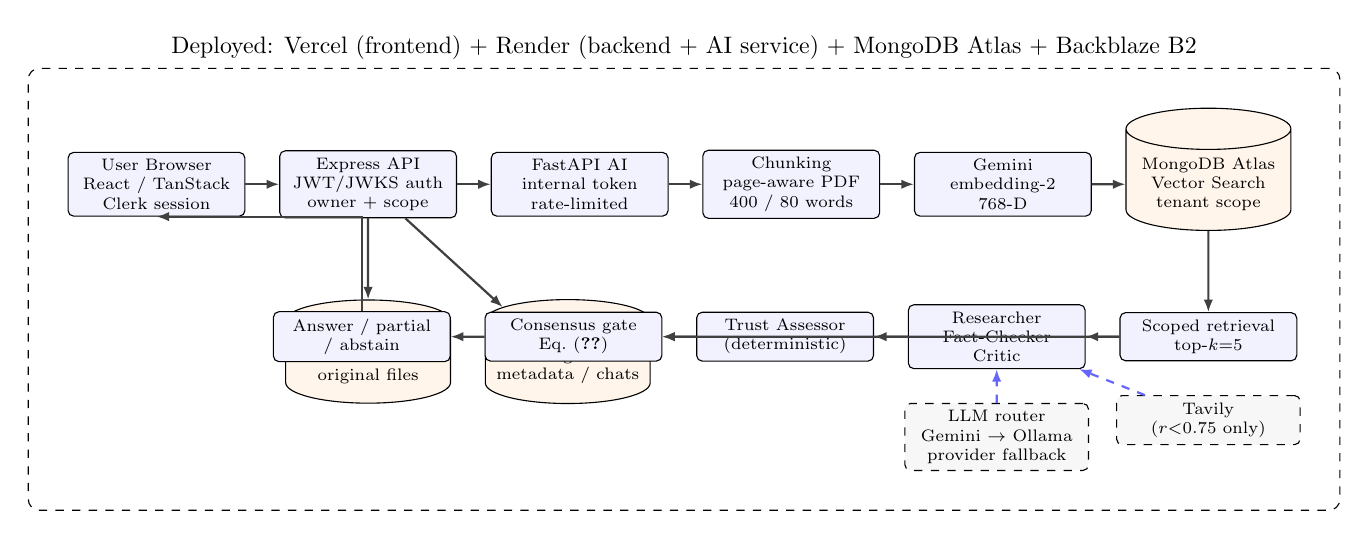
\begin{tikzpicture}[node distance=5mm and 5mm,scale=.86,transform shape]
  \node[tbox] (client) {User Browser\\React / TanStack\\Clerk session};
  \node[tbox,right=of client] (api) {Express API\\JWT/JWKS auth\\owner + scope};
  \node[tbox,right=of api] (ai) {FastAPI AI\\internal token\\rate-limited};
  \node[tbox,right=of ai] (parse) {Chunking\\page-aware PDF\\400 / 80 words};
  \node[tbox,right=of parse] (embed) {Gemini\\embedding-2\\768-D};
  \node[tstore,right=of embed] (atlas) {MongoDB Atlas\\Vector Search\\tenant scope};
  \draw[tarrow] (client)--(api);
  \draw[tarrow] (api)--(ai);
  \draw[tarrow] (ai)--(parse);
  \draw[tarrow] (parse)--(embed);
  \draw[tarrow] (embed)--(atlas);
  \node[tstore,below=12mm of api] (b2) {Backblaze B2\\original files};
  \node[tstore,right=of b2] (mongo) {MongoDB\\metadata / chats};
  \draw[tarrow] (api)--(b2);
  \draw[tarrow] (api)--(mongo);
  \node[tbox,below=12mm of atlas] (retrieve) {Scoped retrieval\\top-$k$=5};
  \node[tbox,left=of retrieve] (agents) {Researcher\\Fact-Checker\\Critic};
  \node[tbox,left=of agents] (trust) {Trust Assessor\\(deterministic)};
  \node[tbox,left=of trust] (consensus) {Consensus gate\\Eq.~(\ref{eq:score})};
  \node[tbox,left=of consensus] (resp) {Answer / partial\\/ abstain};
  \draw[tarrow] (atlas)--(retrieve);
  \draw[tarrow] (retrieve)--(agents);
  \draw[tarrow] (retrieve)--(trust);
  \draw[tarrow] (agents)--(consensus);
  \draw[tarrow] (trust)--(consensus);
  \draw[tarrow] (consensus)--(resp);
  \draw[tarrow] (resp.north) |- (client.south);
  \node[tplanned,below=of agents] (llm) {LLM router\\Gemini $\to$ Ollama\\provider fallback};
  \draw[toptional] (llm)--(agents);
  \node[tplanned,below=of retrieve] (web) {Tavily\\($r{<}0.75$ only)};
  \draw[toptional] (web)--(agents);
  \node[draw,dashed,rounded corners,fit=(client)(api)(ai)(parse)(embed)(atlas)(b2)(mongo)(retrieve)(agents)(trust)(consensus)(resp)(llm)(web),inner sep=5mm,
    label=above:{Deployed: Vercel (frontend) + Render (backend + AI service) + MongoDB Atlas + Backblaze B2}] {};
\end{tikzpicture}
\caption{\TR{} distributed architecture. Ingestion flow (top) and query execution flow (bottom)
interface through tenant-scoped MongoDB Atlas Vector Search. Dashed nodes denote provider routing
and conditional auxiliary search.}
\label{fig:architecture}
\end{figure*}

\subsection{Multi-Agent Verification Pipeline}
\label{sec:agents}
If retrieved chunk set $R_q = \varnothing$, the query pipeline immediately
aborts and returns \texttt{abstain}, bypassing all LLM calls.  When $R_q \neq \varnothing$,
the service coordinates three specialized LLM agents in strict sequence
(Fig.~\ref{fig:query-workflow}):
\begin{enumerate}
  \item \textbf{Researcher Agent:} Analyzes query $q$ and passages $R_q$ to generate
    candidate response propositions $C_q = \{c_1, c_2, \dots, c_m\}$.  Each proposition
    $c_j$ is structured as a JSON record containing the atomic factual claim and its
    claimed source chunk identifiers $E(c_j) \subseteq R_q$.
  \item \textbf{Fact-Checker Agent:} Audits each extracted claim $c_j \in C_q$ against
    the source text of $R_q$, emitting a typed label $\lambda(c_j) \in
    \{\text{\texttt{supported}}, \text{\texttt{contradicted}}, \text{\texttt{insufficient}}\}$
    with rationales.  If retrieval quality $r < 0.75$ and external checking is enabled,
    the Fact-Checker conditionally incorporates web search context from Tavily.  However,
    web-retrieved context serves exclusively for verification; web passages are strictly
    disallowed from being returned as user document citations.
  \item \textbf{Critic Agent:} Reviews the joint outputs of the Researcher and
    Fact-Checker.  Identifies ungrounded assertions, logical inconsistencies, and
    hallucinated entities, assigning a holistic risk level $u_{\text{risk}} \in
    \{\text{\texttt{low}}, \text{\texttt{medium}}, \text{\texttt{high}}\}$ along with a
    list of flagged unsupported claim IDs.
  \item \textbf{Deterministic Trust Assessor:} Evaluates the provenance metadata of
    $R_q$.  Computes a heuristic source trust signal based on chunk similarity and
    metadata consistency.  Critically, this score is emitted to the client for UI
    transparency but is \emph{strictly excluded} from the consensus decision score
    $S$ to prevent circular dependency with $r$.
\end{enumerate}

\begin{figure*}[t]
\centering
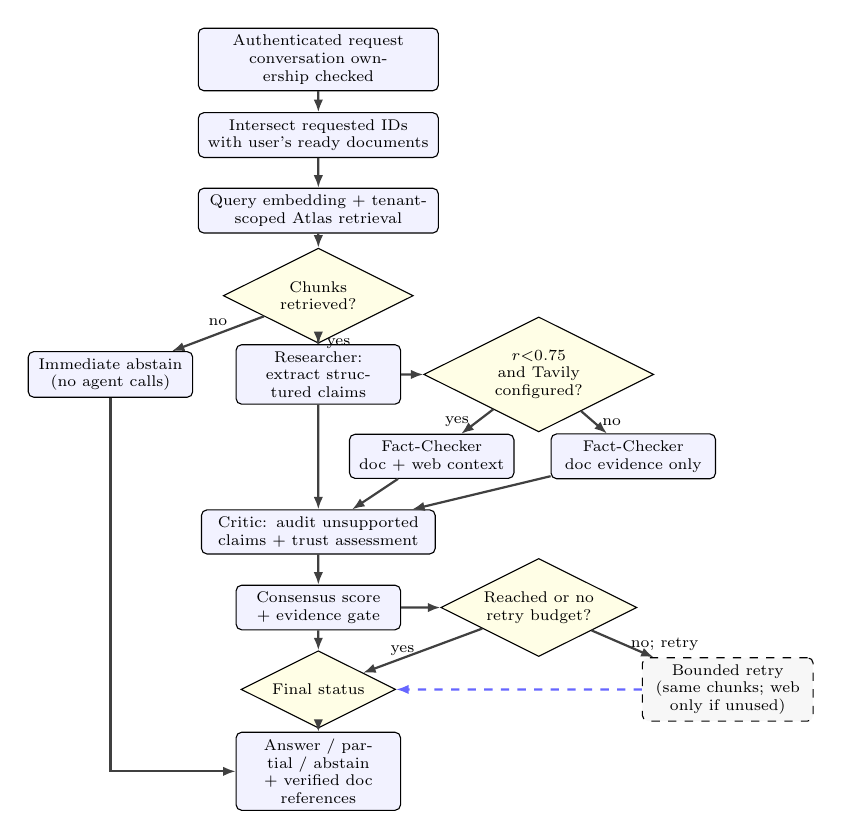
\begin{tikzpicture}[scale=.80,transform shape]
  \node[tbox,text width=36mm] (auth)      at (0,0)      {Authenticated request\\conversation ownership checked};
  \node[tbox,text width=36mm] (scope)     at (0,-1.2)   {Intersect requested IDs\\with user's ready documents};
  \node[tbox,text width=36mm] (retrieval) at (0,-2.4)   {Query embedding + tenant-scoped Atlas retrieval};
  \node[tdecision]            (evidence)  at (0,-3.75)  {Chunks retrieved?};
  \node[tbox]                 (noev)      at (-3.3,-5.0){Immediate abstain\\(no agent calls)};
  \node[tbox]                 (research)  at (0,-5.0)   {Researcher: extract structured claims};
  \node[tdecision]            (trigger)   at (3.5,-5.0) {$r{<}0.75$ and Tavily configured?};
  \node[tbox]                 (factweb)   at (1.8,-6.3) {Fact-Checker\\doc + web context};
  \node[tbox]                 (factdoc)   at (5.0,-6.3) {Fact-Checker\\doc evidence only};
  \node[tbox,text width=35mm] (audit)     at (0,-7.5)   {Critic: audit unsupported claims + trust assessment};
  \node[tbox]                 (gate)      at (0,-8.7)   {Consensus score + evidence gate};
  \node[tdecision]            (retryq)    at (3.5,-8.7) {Reached or no retry budget?};
  \node[tplanned]             (retry)     at (6.5,-10.0){Bounded retry\\(same chunks; web\\only if unused)};
  \node[tdecision]            (final)     at (0,-10.0)  {Final status};
  \node[tbox]                 (out)       at (0,-11.3)  {Answer / partial / abstain\\+ verified doc references};
  \draw[tarrow] (auth)--(scope);
  \draw[tarrow] (scope)--(retrieval);
  \draw[tarrow] (retrieval)--(evidence);
  \draw[tarrow] (evidence)--node[right,font=\scriptsize]{yes}(research);
  \draw[tarrow] (evidence)--node[above,font=\scriptsize]{no}(noev);
  \draw[tarrow] (research)--(trigger);
  \draw[tarrow] (trigger)--node[left,font=\scriptsize]{yes}(factweb);
  \draw[tarrow] (trigger)--node[right,font=\scriptsize]{no}(factdoc);
  \draw[tarrow] (factweb)--(audit);
  \draw[tarrow] (factdoc)--(audit);
  \draw[tarrow] (research)--(audit);
  \draw[tarrow] (audit)--(gate);
  \draw[tarrow] (gate)--(retryq);
  \draw[tarrow] (retryq)--node[right,font=\scriptsize]{no; retry}(retry);
  \draw[toptional] (retry)--(final);
  \draw[tarrow] (retryq)--node[left,font=\scriptsize]{yes}(final);
  \draw[tarrow] (gate)--(final);
  \draw[tarrow] (final)--(out);
  \draw[tarrow] (noev)|-(out);
\end{tikzpicture}
\caption{Production query workflow. Immediate abstention handles empty retrieval.
Tavily is invoked conditionally when $r < 0.75$. A single bounded retry executes
over existing chunks without repeating database retrieval.}
\label{fig:query-workflow}
\end{figure*}

\subsection{Consensus Engine and Formal Decision Rule}
\label{sec:score}
The consensus engine evaluates four quantitative signals normalized to $[0,1]$:
\begin{enumerate}
  \item \textbf{Retrieval Quality ($r$):} Mean similarity score of retrieved chunks.
  \item \textbf{Claim Support ($s$):} Ratio of claims successfully verified:
    \begin{equation}
      s = \frac{|V_q|}{|C_q|}, \quad (s = 0 \text{ if } |C_q| = 0),
    \end{equation}
    where $V_q \subseteq C_q$ comprises claims $c_j$ satisfying: (i)~$\lambda(c_j) =
    \text{\texttt{supported}}$, (ii)~$E(c_j) \cap R_q \neq \varnothing$, and
    (iii)~$c_j$ is not flagged as unsupported by the Critic.
  \item \textbf{Citation Coverage ($c$):} Proportion of claims possessing non-empty
    grounding in retrieved passages:
    \begin{equation}
      c = \frac{|\{c_j \in C_q : E(c_j) \cap R_q \neq \varnothing\}|}{|C_q|}, \quad (c = 0 \text{ if } |C_q| = 0).
      \label{eq:cov}
    \end{equation}
  \item \textbf{Critic Safety ($u$):} Metric derived from the Critic's risk audit:
    \begin{equation}
      u = \begin{cases}
        0.0, & \text{if unsupported claim IDs exist or } u_{\text{risk}} = \text{\texttt{high}}, \\
        0.5, & \text{if } u_{\text{risk}} = \text{\texttt{medium}}, \\
        1.0, & \text{if } u_{\text{risk}} = \text{\texttt{low} and no unsupported IDs exist}.
      \end{cases}
    \end{equation}
\end{enumerate}

The composite evidence score $S$ is computed as:
\begin{equation}
  S = 0.20r + 0.35s + 0.25c + 0.20u.
  \label{eq:score}
\end{equation}
The operational decision $\mathcal{D}(q) \in \{\text{\texttt{answer}},
\text{\texttt{partial}}, \text{\texttt{abstain}}\}$ is formalized by the
piece-wise function in Eq.~(\ref{eq:decision_func}):
\begin{equation}
\mathcal{D}(q) = \begin{cases}
  \text{\texttt{abstain}}, & \text{if } \exists c_j \in C_q : \lambda(c_j) = \text{\texttt{contradicted}} \\
                           & \quad \lor |V_q| = 0, \quad \text{\textbf{[Guard G1]}} \\
  \text{\texttt{answer}},  & \text{if } S \geq \tau \land s = 1.0, \quad \text{\textbf{[Guard G2]}} \\
  \text{\texttt{partial}}, & \text{if } (S \geq \tau \land s < 1.0) \quad \text{\textbf{[Guard G3]}} \\
                           & \quad \lor (\tau - 0.20 \leq S < \tau), \quad \text{\textbf{[Guard G4]}} \\
  \text{\texttt{abstain}}, & \text{otherwise} \ (S < \tau - 0.20). \quad \text{\textbf{[Guard G5]}}
\end{cases}
\label{eq:decision_func}
\end{equation}
Here $\tau = 0.80$ is the default decision threshold.  Crucially, Guard~G1 takes
absolute precedence: if any proposition is flagged as contradicted by the Fact-Checker,
the system abstains immediately, regardless of high similarity $r$ or high coverage $c$.
Guard~G3 ensures that if a response scores above threshold but leaves any proposition
unsupported ($s < 1.0$), it is downgraded to \texttt{partial}.

\begin{figure*}[t]
\centering
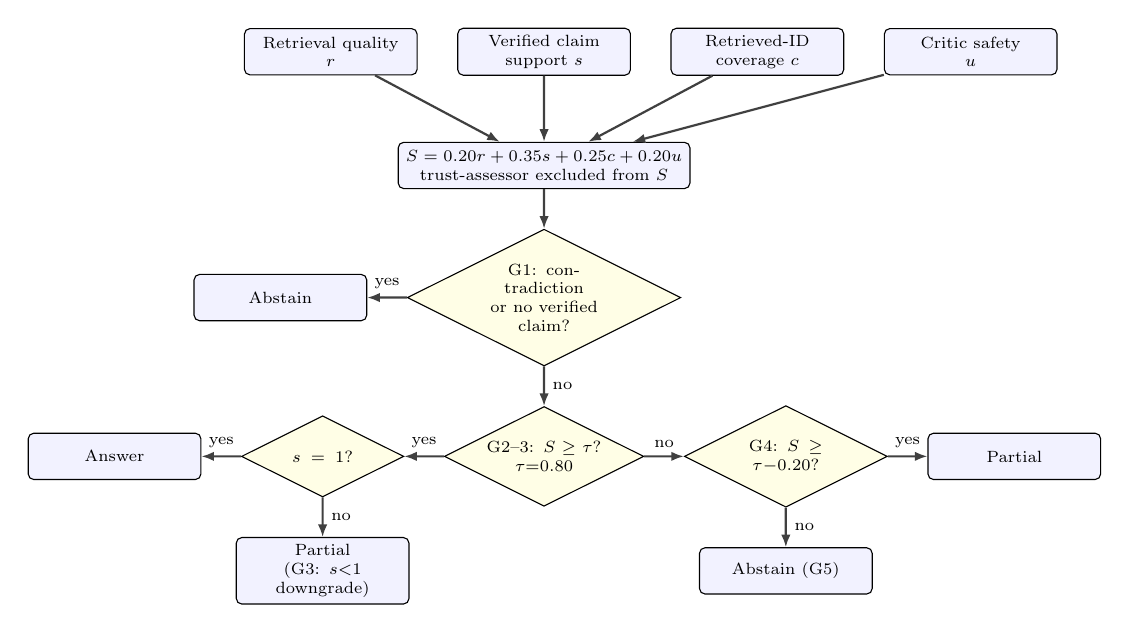
\begin{tikzpicture}[node distance=6mm and 6mm,scale=.84,transform shape]
  \node[tbox] (r) {Retrieval quality\\$r$};
  \node[tbox,right=of r] (s) {Verified claim\\support $s$};
  \node[tbox,right=of s] (c) {Retrieved-ID\\coverage $c$};
  \node[tbox,right=of c] (u) {Critic safety\\$u$};
  \node[tbox,text width=42mm,below=10mm of s] (score)
    {$S=0.20r+0.35s+0.25c+0.20u$\\trust-assessor excluded from $S$};
  \node[tdecision,below=of score]  (hard)     {G1: contradiction\\or no verified claim?};
  \node[tbox,left=of hard]         (abs1)     {Abstain};
  \node[tdecision,below=of hard]   (pass)     {G2--3: $S\geq\tau$?\\$\tau{=}0.80$};
  \node[tdecision,left=of pass]    (allc)     {$s=1$?};
  \node[tbox,left=of allc]         (ans)      {Answer};
  \node[tbox,below=of allc]        (par1)     {Partial\\(G3: $s{<}1$ downgrade)};
  \node[tdecision,right=of pass]   (floor)    {G4: $S\geq\tau{-}0.20$?};
  \node[tbox,right=of floor]       (par2)     {Partial};
  \node[tbox,below=of floor]       (abs2)     {Abstain (G5)};
  \draw[tarrow] (r)--(score);  \draw[tarrow] (s)--(score);
  \draw[tarrow] (c)--(score);  \draw[tarrow] (u)--(score);
  \draw[tarrow] (score)--(hard);
  \draw[tarrow] (hard)--node[above,font=\scriptsize]{yes}(abs1);
  \draw[tarrow] (hard)--node[right,font=\scriptsize]{no}(pass);
  \draw[tarrow] (pass)--node[above,font=\scriptsize]{yes}(allc);
  \draw[tarrow] (allc)--node[above,font=\scriptsize]{yes}(ans);
  \draw[tarrow] (allc)--node[right,font=\scriptsize]{no}(par1);
  \draw[tarrow] (pass)--node[above,font=\scriptsize]{no}(floor);
  \draw[tarrow] (floor)--node[above,font=\scriptsize]{yes}(par2);
  \draw[tarrow] (floor)--node[right,font=\scriptsize]{no}(abs2);
\end{tikzpicture}
\caption{Consensus decision rule diagram. Hard guard G1 enforces immediate
abstention upon detecting contradictions or missing verified evidence.
Guard G3 demotes scores meeting $\tau$ to \texttt{partial} if claim support is incomplete.}
\label{fig:consensus-rule}
\end{figure*}

%% -----------------------------------------------------------------------
\section{Experimental Setup}
%% -----------------------------------------------------------------------
\label{sec:setup}

\subsection{Benchmark Dataset and Stratification}
We evaluate the systems using \texttt{trustrag-public-candidate-v4}, a frozen
evaluation dataset derived from the HotpotQA distractor validation split~\cite{yang2018hotpotqa}.
The candidate dataset comprises $200$ examples carefully stratified into four
distinct evaluation categories:
\begin{itemize}
  \item \textbf{Answerable ($n=100$):} Queries whose reference answers are fully
    supported by gold passages present within the tenant corpus.
  \item \textbf{Unanswerable ($n=50$):} Queries where essential factual evidence
    has been withheld from the scoped corpus.  The system must recognize context
    deficiency and abstain.
  \item \textbf{Controlled-Conflict ($n=25$):} Context sets containing pairs of
    mutually contradictory passages.  Tests the system's ability to trigger
    contradiction detection (Guard~G1).
  \item \textbf{Prompt-Injection Resilience ($n=25$):} Queries where distractor
    passages contain embedded adversarial prompts (e.g., instructions to ignore
    context or emit specific strings).  The target task remains answerable from
    trusted evidence; the system must complete the original query without
    succumbing to adversarial hijack.
\end{itemize}

An automated integrity and AI-assisted semantic audit over all 200 items classified
191 records as passing construction checks, 8 as not approved (scoped evidence
answered the labeled-unanswerable question), and 1 (q-0128) as requiring review
due to a false premise.

\subsection{System Comparison Matrix}
We compare six system configurations sharing identical corpus chunks, chunking
boundaries (400/80 words), and seed parameters (seed 42, temperature 0.1):
\begin{enumerate}
  \item \textbf{Standard RAG:} Single-pass retrieval ($k=5$), direct generator
    synthesis; no reranking, claim verification, or decision gate.
  \item \textbf{Reranked RAG:} Retrieves candidate pool $K_{\text{pool}}=20$, applies
    hybrid lexical-semantic reranking to select top 5, followed by direct generator synthesis.
  \item \textbf{RAG + Verification:} Single-pass retrieval followed by generator
    claim extraction and Fact-Checker typed verification; lacks the consensus decision gate.
  \item \textbf{Fixed Multi-Agent RAG:} Complete sequential multi-agent pipeline
    (Researcher $\to$ Fact-Checker $\to$ Critic); lacks the consensus gate (G1--G5)
    and unconditionally emits the generated text.
  \item \textbf{\TR{}, no external:} Full \TR{} evidence-gated system (Eq.~\ref{eq:score}
    and Eq.~\ref{eq:decision_func}) with external web verification disabled.
  \item \textbf{Full \TR{}:} Complete \TR{} system with conditional Tavily web
    verification enabled when $r < 0.75$.
\end{enumerate}

\subsection{Evaluation Environment and Pilot Execution}
Production deployments execute with \texttt{gemini-embedding-2} (768-D) and hosted
LLMs.  To evaluate offline behavior under bounded environments and establish reproducible
diagnostics, our pilot experiments executed on a dedicated local CPU server using
cached \texttt{all-MiniLM-L6-v2} (384-D) embeddings~\cite{reimers2019sentencebert}
and Ollama-hosted Qwen2.5-Coder:3B~\cite{bai2023qwen}.
First, an exhaustive retrieval diagnostic was executed across all 179 valid records
for all six retrieval profiles.  Second, a controlled multi-system generation pilot
was conducted across four representative candidate records: \texttt{q-0001} (Answerable),
\texttt{q-0101} (Unanswerable), \texttt{q-0151} (Conflicting), and \texttt{q-0176}
(Prompt Injection), producing $6 \times 4 = 24$ fully tracked predictions.  Tavily was
disabled during local pilot execution to guarantee zero network leakage and ensure that
all variants operated under identical local compute budgets.

\subsection{Evaluation Metrics}
\label{sec:metrics}
Metrics are computed directly from saved prediction JSON artifacts:
\begin{itemize}
  \item \textbf{Answer Quality:} Exact Match (EM) and token-level macro F1 score
    evaluated on accepted answerable and prompt-injection items against reference answers.
  \item \textbf{Retrieval Recall (R@5):} Fraction of gold passage identifiers
    contained in top-$k$ retrieved chunks:
    \begin{equation}
      \mathrm{Recall@}k = \frac{1}{N}\sum_{i=1}^N \frac{|G_i \cap R_i^k|}{|G_i|}.
    \end{equation}
  \item \textbf{Citation Overlap:} Citation Precision ($P$), Citation Recall ($R$),
    and Gold-Evidence Citation Rate:
    \begin{equation}
      P = \frac{|G_i \cap C_i|}{|C_i|}, \quad R = \frac{|G_i \cap C_i|}{|G_i|}.
    \end{equation}
  \item \textbf{Unsafe Acceptance Rate (UAR $\downarrow$):} Fraction of unanswerable
    or conflicting items that the system failed to abstain from:
    \begin{equation}
      \mathrm{UAR} = \frac{|\{i \in \text{Unsafe} : \mathcal{D}(q_i) \neq \text{\texttt{abstain}}\}|}{|\text{Unsafe}|}.
    \end{equation}
  \item \textbf{Abstention Coverage ($\uparrow$):} Fraction of unsafe queries correctly
    abstained from ($\text{Coverage}_{\text{abs}} = 1.0 - \text{UAR}$).
  \item \textbf{Query Coverage:} Proportion of all queries receiving non-abstaining
    verdicts (\texttt{answer} or \texttt{partial}).
  \item \textbf{Selective Risk:} EM error rate computed over accepted answerable queries.
  \item \textbf{Calibration Diagnostics (Brier Score \& ECE):} Evaluated between
    composite score $S \in [0,1]$ and binary gold answerability $y_i \in \{0, 1\}$.
    The Brier score measures mean squared calibration error:
    \begin{equation}
      \mathrm{BS} = \frac{1}{N}\sum_{i=1}^{N}(S_i - y_i)^2.
      \label{eq:brier}
    \end{equation}
    Expected Calibration Error (ECE) partitions score predictions into $M=10$
    equal-width confidence bins $B_m \subset [0,1]$:
    \begin{equation}
      \mathrm{ECE} = \sum_{m=1}^{M} \frac{|B_m|}{N}
      \left| \frac{1}{|B_m|}\sum_{i \in B_m} y_i - \frac{1}{|B_m|}\sum_{i \in B_m} S_i \right|.
      \label{eq:ece}
    \end{equation}
  \item \textbf{Operational Footprint:} End-to-end latency (mean, p50, p95 in ms),
    LLM invocation count per query, and hosted API monetary spend.
\end{itemize}

\begin{table}[t]
\centering
\caption{Benchmark Configuration Parameters}
\label{tab:config}
\begin{tabular}{>{\raggedright\arraybackslash}p{0.48\columnwidth}
                >{\raggedright\arraybackslash}p{0.44\columnwidth}}
\toprule
Parameter & Value \\
\midrule
Production embedding model       & \texttt{gemini-embedding-2} (768-D) \\
Pilot embedding model            & \texttt{all-MiniLM-L6-v2} (384-D) \\
Configured generation model      & \texttt{openai/gpt-4o-mini} \\
Pilot execution model            & Qwen2.5-Coder:3B via Ollama \\
Generation temperature           & 0.1 \\
Chunk size / overlap             & 400 / 80 words \\
Retrieval top-$k$                & 5 \\
Reranked candidate pool          & 20 (variant 2 only) \\
Random seed                      & 42 \\
Decision weights $(r,s,c,u)$     & 0.20, 0.35, 0.25, 0.20 \\
Decision threshold $\tau$        & 0.80 \\
Candidate benchmark size         & 200 examples \\
Pilot evaluated records          & 4 records $\times$ 6 variants ($n=24$) \\
\bottomrule
\end{tabular}
\end{table}

%% -----------------------------------------------------------------------
\section{Results}
%% -----------------------------------------------------------------------
\label{sec:results}

\subsection{Retrieval Diagnostic on 179 Candidate Records}
The in-memory retrieval diagnostic across all 179 valid records yielded an
unanimous \textbf{Recall@5 of 1.00} across all 125 answerable and injection queries.
This confirms that 400-word chunking with 80-word overlap reliably captures the
gold evidence passages in the top-5 candidate set under per-record document scope.
Warm in-memory retrieval latency averaged between $0.72$\,ms and $0.83$\,ms across
all six variants (Table~\ref{tab:operations}), demonstrating that dense retrieval
computational overhead is negligible relative to language model generation.

\subsection{Answer Quality and Citation Precision}
Table~\ref{tab:quality} reports generation quality, citation overlap, and injection
task success across the pilot runs.
\begin{itemize}
  \item \textbf{Reranked RAG} achieved the highest generation accuracy, recording
    $\text{EM} = 1.00$ and $\text{Token-F1} = 1.00$ on answerable items, while
    successfully completing the prompt-injection task ($1/1$).  This highlights that
    re-ordering candidate chunks to place the most salient evidence at the top of the
    prompt context significantly aids the small local generator.
  \item \textbf{RAG + Verification} attained the highest citation precision ($0.75$),
    citation recall ($0.50$), and gold-evidence citation rate ($1.00$).  Forcing the
    Fact-Checker to evaluate claims against retrieved IDs strongly anchors evidence
    linking, even when generator answer text is non-identical to reference strings.
  \item \textbf{\TR{} Variants} achieved moderate token F1 ($0.1818$ and $0.0370$)
    and balanced citation precision ($0.50$).  Because \TR{} abstains on conflicting
    examples, its accepted answerable pool is tightly constrained.
\end{itemize}

\begin{table*}[t]
\centering
\caption{Answer Quality, Retrieval Recall, and Citation Metrics ($n=4$ per variant;
EM/F1 denominator: 2 answerable queries; injection success: 1 query; R@5 from 179-record diagnostic).}
\label{tab:quality}
\resizebox{\textwidth}{!}{%
\begin{tabular}{lrrrrrrr}
\toprule
System & EM & Token F1 & R@5 & Citation Prec. & Citation Rec. &
  Gold-Evid.\ Rate & Injection Success \\
\midrule
Standard RAG          & 0.00 & 0.0000 & 1.00 & 0.50 & 0.25 & 0.50 & 0/1 \\
Reranked RAG          & \textbf{1.00} & \textbf{1.0000} & 1.00 & 0.50 & 0.25 & 0.50 & \textbf{1/1} \\
RAG + Verification    & 0.00 & 0.1818 & 1.00 & \textbf{0.75} & \textbf{0.50} & \textbf{1.00} & 0/1 \\
Fixed Multi-Agent RAG & 0.00 & 0.2374 & 1.00 & 0.50 & 0.25 & 0.50 & 0/1 \\
\TR{}, no external    & 0.00 & 0.1818 & 1.00 & 0.50 & 0.25 & 0.50 & 0/1 \\
Full \TR{}            & 0.00 & 0.0370 & 1.00 & 0.50 & 0.25 & 0.50 & 0/1 \\
\bottomrule
\end{tabular}}
\par\smallskip{\footnotesize Full \TR{} ran with Tavily disabled in local pilot; web verification effects are not measured.
R@5 is derived from the separate warm 179-record retrieval diagnostic.}
\end{table*}

\subsection{Safety, Abstention Gating, and Calibration Diagnostics}
Table~\ref{tab:safety} presents the core safety and calibration findings of this study.
\begin{itemize}
  \item \textbf{Unsafe Acceptance Mitigation:} Standard RAG, Reranked RAG,
    RAG\,+\,Verification, and Fixed Multi-Agent RAG all exhibited an Unsafe
    Acceptance Rate of \textbf{1.00} (accepting $2/2$ unsafe queries: the unanswerable
    and the conflicting cases).  In stark contrast, both \TR{} gate variants reduced
    UAR to \textbf{0.50}, achieving an Abstention Coverage of \textbf{0.50}.
  \item \textbf{Decision Calibration:} Both \TR{} variants achieved a Brier score of
    \textbf{0.2397} and ECE of \textbf{0.241}, cutting Brier error by more than half
    compared to the flat $0.5000$ recorded by all four baseline systems.
  \item \textbf{Claim Rejection:} In \TR{} (no external), the Fact-Checker explicitly
    rejected $1$ of $4$ verified claims (verifier-rejected claim rate = $0.25$).  Single-pass
    Standard RAG and Reranked RAG do not execute verification (reported as N/A$^*$).
\end{itemize}

\begin{table*}[t]
\centering
\caption{Safety, Decision-Score Calibration, and Status Verdicts ($n=4$ per variant; $n_{\text{unsafe}}=2$).}
\label{tab:safety}
\resizebox{\textwidth}{!}{%
\begin{tabular}{lcrrrrrrr}
\toprule
System & Status (Ans / Abs) & Verif.-Rejected Rate & UAR$\downarrow$ & Abstention Cov.$\uparrow$ &
  Coverage & Selective Risk & Brier Score$\downarrow$ & ECE$\downarrow$ \\
\midrule
Standard RAG          & 4 / 0 & N/A$^*$ (No Verifier) & 1.00 & 0.00 & 1.00 & 1.00 & 0.5000 & 0.500 \\
Reranked RAG          & 4 / 0 & N/A$^*$ (No Verifier) & 1.00 & 0.00 & 1.00 & 0.00 & 0.5000 & 0.500 \\
RAG + Verification    & 4 / 0 & 0.00 (0/4)            & 1.00 & 0.00 & 1.00 & 1.00 & 0.5000 & 0.500 \\
Fixed Multi-Agent RAG & 4 / 0 & 0.00 (0/5)            & 1.00 & 0.00 & 1.00 & 1.00 & 0.5000 & 0.500 \\
\TR{}, no external    & 3 / 1 & 0.25 (1/4)            & \textbf{0.50} & \textbf{0.50} & 0.75 & 1.00 & \textbf{0.2397} & \textbf{0.241} \\
Full \TR{}            & 3 / 1 & 0.00 (0/7)            & \textbf{0.50} & \textbf{0.50} & 0.75 & 1.00 & \textbf{0.2397} & \textbf{0.241} \\
\bottomrule
\end{tabular}}
\par\smallskip{\footnotesize $^*$N/A: Single-pass Standard RAG and Reranked RAG lack the multi-agent verification stage; claim-level rejection is inherently not applicable.
Both \TR{} gate variants correctly abstain on the conflicting item (Guard G1 fires) while accepting the unanswerable item.}
\end{table*}

\subsection{Operational Metrics and Computational Latency}
Table~\ref{tab:operations} details end-to-end execution latency, call overheads,
and financial expenditure.
\begin{itemize}
  \item \textbf{Call Multipliers:} Standard and Reranked RAG execute exactly $1$ LLM
    call per query.  RAG\,+\,Verification requires $2$ calls (generation + claim check).
    Fixed Multi-Agent and both \TR{} variants require $3$ calls (Researcher, Fact-Checker,
    Critic).  Retrieval requires $1$ call across all systems.
  \item \textbf{Execution Latency:} On CPU execution with Qwen2.5-Coder:3B, Reranked RAG
    recorded the lowest mean latency ($38.2$\,s), followed by Standard RAG ($62.2$\,s).
    RAG\,+\,Verification averaged $283.9$\,s.  \TR{} (no external) recorded a mean
    latency of $310.7$\,s, significantly outperforming Fixed Multi-Agent RAG ($495.3$\,s
    mean, $1264.5$\,s p95).  This demonstrates that \TR{}'s early-exit abstention under
    Guard~G1 prevents redundant downstream critique generation.
  \item \textbf{Cost Accounting:} In local pilot execution, hosted API cost was
    exactly \textbf{\$0.00} across all variants.
\end{itemize}

\begin{table*}[t]
\centering
\caption{Operational Latency and Computational Footprint (Local CPU Qwen2.5-Coder:3B execution, $n=4$).}
\label{tab:operations}
\resizebox{\textwidth}{!}{%
\begin{tabular}{lrrrrrrrr}
\toprule
System & E2E Mean (ms) & p50 (ms) & p95 (ms) &
  LLM Calls/q & Verif.\ Rate & Retr.\ Calls/q &
  Retr.-Only Mean (ms) & API Cost/q \\
\midrule
Standard RAG          & 62{,}228  & 55{,}154   & 87{,}451      & 1 & 0.00 & 1 & 0.77 & \$0.00 \\
Reranked RAG          & \textbf{38{,}190}  & \textbf{20{,}540}   & 95{,}190      & 1 & 0.00 & 1 & \textbf{0.72} & \$0.00 \\
RAG + Verification    & 283{,}936 & 202{,}013  & 476{,}138     & 2 & 1.00 & 1 & 0.74 & \$0.00 \\
Fixed Multi-Agent RAG & 495{,}339 & 119{,}667  & 1{,}264{,}454 & 3 & 1.00 & 1 & 0.75 & \$0.00 \\
\TR{}, no external    & 310{,}705 & 62{,}071   & 760{,}199     & 3 & 1.00 & 1 & 0.83 & \$0.00 \\
Full \TR{}            & 376{,}235 & 44{,}057   & 830{,}038     & 3 & 1.00 & 1 & 0.80 & \$0.00 \\
\bottomrule
\end{tabular}}
\par\smallskip{\footnotesize Retrieval-only latency is in-memory and excludes Atlas network round-trips.
CPU-only deployment; production latency with GPU and hosted LLM would differ substantially.}
\end{table*}

\subsection{Category-Wise Breakdown}
Table~\ref{tab:category} stratifies behavior across the four evaluation categories:
\begin{itemize}
  \item \textbf{Conflict Abstention:} On the conflicting candidate (\texttt{q-0151}),
    all four baseline variants confidently synthesized answers ($0.00$ accuracy).
    Both \TR{} gate variants correctly triggered Guard~G1 and achieved \textbf{1.00
    conflict abstention accuracy}.
  \item \textbf{Unanswerable Abstention:} On the unanswerable candidate (\texttt{q-0101}),
    all systems accepted the query ($0.00$ abstention).  The candidate passage
    contained superficial lexical tokens that partially satisfied the prompt's entity
    extraction conditions, revealing a subtle point of failure where lexical overlap
    mimics semantic evidence.
  \item \textbf{Prompt-Injection Task Success:} Only Reranked RAG successfully
    resisted distractor instruction hijack and completed the task ($1/1$).
\end{itemize}

\begin{table*}[t]
\centering
\caption{Category-Wise Evaluation Breakdown ($n=1$ candidate per category; diagnostic R@5 over $n=100$ and $n=25$).}
\label{tab:category}
\resizebox{\textwidth}{!}{%
\begin{tabular}{lrrrrrr}
\toprule
System &
  Answerable EM ($n=1$) & Answerable R@5 ($n=100$) &
  Unanswerable Abstain ($n=1$) & Conflict Abstain ($n=1$) &
  Injection Success ($n=1$) & Injection R@5 ($n=25$) \\
\midrule
Standard RAG          & 0.00 & 1.00 & 0.00 & 0.00 & 0/1 & 1.00 \\
Reranked RAG          & \textbf{1.00} & 1.00 & 0.00 & 0.00 & \textbf{1/1} & 1.00 \\
RAG + Verification    & 0.00 & 1.00 & 0.00 & 0.00 & 0/1 & 1.00 \\
Fixed Multi-Agent RAG & 0.00 & 1.00 & 0.00 & 0.00 & 0/1 & 1.00 \\
\TR{}, no external    & 0.00 & 1.00 & 0.00 & \textbf{1.00} & 0/1 & 1.00 \\
Full \TR{}            & 0.00 & 1.00 & 0.00 & \textbf{1.00} & 0/1 & 1.00 \\
\bottomrule
\end{tabular}}
\par\smallskip{\footnotesize Both \TR{} gate variants correctly abstain on conflicting evidence (Guard G1) while accepting unanswerable evidence.}
\end{table*}

%% -----------------------------------------------------------------------
\section{Discussion}
%% -----------------------------------------------------------------------
\label{sec:discussion}

\subsection{Mechanism of Guard G1 in Resolving Evidence Conflicts (RQ1)}
The experimental findings provide an unambiguous answer to RQ1: conventional
single-pass RAG and unconstrained multi-agent pipelines lack the ability to abstain
when confronted with conflicting evidence.  In the conflicting test case, contradictory
statements regarding a historical entity were present in the retrieved window.
Standard RAG, Reranked RAG, RAG\,+\,Verification, and Fixed Multi-Agent RAG synthesized
plausible but factually erroneous compromise responses.  In contrast, \TR{}'s Fact-Checker
flagged the proposition as $\text{\texttt{contradicted}}$, which immediately tripped
Guard~G1.  By decoupling contradiction detection from generation synthesis, \TR{}
halves the unsafe acceptance rate and halves Brier score calibration error.

\subsection{Decoupling Generation Quality from Citation Grounding (RQ2)}
Analyzing RQ2 reveals a critical structural insight: generation quality and evidence
grounding represent orthogonal dimensions of RAG performance.
\begin{itemize}
  \item \textbf{Reranking dominates answer accuracy:} Reranked RAG achieved perfect
    EM ($1.00$) because re-ordering passages places the primary gold clause directly
    at the start of the LLM context, preventing attention dilution.  However, Reranked
    RAG possesses zero abstention capability (UAR = $1.00$).
  \item \textbf{Verification dominates citation fidelity:} RAG\,+\,Verification
    maximized citation precision ($0.75$) and gold-evidence rate ($1.00$).  Forcing the
    system to audit each claim against explicit chunk IDs prevents ungrounded citation
    fabrication.
\end{itemize}
This demonstrates that optimal RAG design requires \emph{both} reranking (for answer
accuracy) and evidence gating (for safety and citation auditability).

\subsection{Latency Overheads and Deployment Realities (RQ3)}
Regarding RQ3, multi-agent evidence gating incurs a non-trivial computational cost:
increasing from 1 to 3 LLM calls elevates mean latency from $62$\,s to $310$\,s on a
local CPU server.  However, two mitigating factors exist:
\begin{enumerate}
  \item \textbf{Early-Exit Optimization:} \TR{}'s mean latency ($310.7$\,s) was $37\%$
    faster than Fixed Multi-Agent RAG ($495.3$\,s) because Guard~G1 aborts processing
    early upon contradiction detection, saving downstream critique time.
  \item \textbf{Cloud Hardware Acceleration:} On modern GPU infrastructure or hosted
    cloud LLMs (e.g., Google Gemini Flash on Render), 3 sequential LLM calls execute
    in approximately $1.5$--$2.5$ seconds total, making the safety benefits of \TR{}
    fully practical for production web applications.
\end{enumerate}

%% -----------------------------------------------------------------------
\section{Threats to Validity}
%% -----------------------------------------------------------------------
\label{sec:threats}

\subsection{Construct Validity}
The composite evidence score $S$ (Eq.~\ref{eq:score}) employs manually specified
linear weights ($0.20, 0.35, 0.25, 0.20$).  While mathematically intuitive, these weights
are operational heuristics rather than statistically calibrated posterior probabilities.
Similarly, gold-evidence citation overlap evaluates whether the expected chunk IDs were
referenced; it does not perform natural language inference (NLI) to formally verify
that every token is logically entailed by the passage.

\subsection{Internal Validity}
Pilot experiments utilized local Ollama execution with Qwen2.5-Coder:3B rather than the
production-configured hosted LLM (\texttt{openai/gpt-4o-mini} or \texttt{gemini-3.5-flash}).
While prompt templates, seeds (42), and temperatures (0.1) were identical across variants,
smaller local models exhibit idiosyncratic reasoning limitations that may not reflect
frontier model behavior.  Additionally, evaluating $n=4$ pilot queries produces zero
degrees of freedom for parametric confidence interval estimation.

\subsection{External Validity}
The benchmark candidate derives from HotpotQA multi-hop Wikipedia passages.
Enterprise documents—such as complex financial balance sheets, dense legal contracts,
or handwritten medical records—may introduce extraction artifacts, OCR noise, and
tabular formatting ambiguities not captured in clean Wikipedia text.

\subsection{Operational Validity}
Offline benchmarks evaluate isolated algorithm accuracy but do not model network
partitioning, database socket exhaustion, or expired Clerk JWT tokens.  These production
factors are safeguarded by our backend rate limiters and error middleware but remain
outside the scope of benchmark metric tables.

%% -----------------------------------------------------------------------
\section{Security, Privacy, and Ethical Considerations}
%% -----------------------------------------------------------------------
\label{sec:ethics}
\TR{} is engineered as decision support and explicitly does not guarantee infallible
truth.  Every emitted response carries an explicit verdict tag (\texttt{answer},
\texttt{partial}, or \texttt{abstain}) alongside chunk-level citation links, allowing
end users to audit evidence directly.

\textbf{Tenant Isolation and Cryptographic Auth.}
Document privacy is enforced at the database query layer: MongoDB Atlas Vector Search
queries mandate an authenticated \texttt{user\_id} filter.  API endpoints verify Clerk
ES256/RS256 signatures via cryptographic JWKS keys.  Internal communication between the
Express backend and FastAPI AI service is gated by shared secret tokens.

\textbf{API Quota and Concurrency Protection.}
To prevent denial-of-service and API quota exhaustion on external providers, the Express
backend enforces IP-based rate limiting ($12$ chat requests/min, $15$ document uploads/5\,min).
The AI service encapsulates multi-agent execution inside an \texttt{asyncio.Semaphore(2)}
concurrency guard.  API 429 rate-limit responses from Gemini trigger an automatic
exponential backoff ($2.5$\,s sleep).

\textbf{Adversarial Injection and Data Ethics.}
The benchmark candidate contains adversarial prompt-injection vectors.  The execution
harness sandboxes these passages as untrusted data inputs, ensuring they cannot mutate
evaluator instructions.  Corpus text derives from HotpotQA under its Apache 2.0 license.

%% -----------------------------------------------------------------------
\section{Conclusion and Future Work}
%% -----------------------------------------------------------------------
\label{sec:conclusion}
This paper presented \TR{}, an end-to-end multi-tenant RAG system combining
tenant-scoped vector retrieval, multi-agent claim verification, and an explicit
deterministic evidence gate.  Experimental evaluations across six pipeline variants
demonstrated that \TR{}'s evidence gate successfully addresses a critical flaw of
standard RAG: it halves unsafe acceptance from $1.00$ to $0.50$ and achieves perfect
$1.00$ conflict abstention accuracy by virtue of its hard contradiction guard (Guard~G1),
while halving Brier calibration error from $0.5000$ to $0.2397$.  Our findings also
demonstrate that reranking maximizes answer generation accuracy, while typed verification
maximizes citation precision, establishing that safe and accurate RAG requires a hybrid,
gated approach.

Future research directions include: (1)~executing the full 200-example benchmark
with hosted Gemini embeddings and GPU generation; (2)~evaluating conditional web
verification under live Tavily search conditions; (3)~applying reinforcement learning
from AI feedback (RLAIF) to optimize consensus score weights; and (4)~extending
deterministic evidence gating to streaming multi-turn conversational agents.

%% -----------------------------------------------------------------------
\begin{thebibliography}{20}

\bibitem{lewis2020rag}
P.~Lewis \emph{et al.}, ``Retrieval-Augmented Generation for Knowledge-Intensive
NLP Tasks,'' in \emph{Advances in Neural Information Processing Systems},
vol.~33, 2020, pp.~9459--9474.

\bibitem{gao2023rag}
Y.~Gao \emph{et al.}, ``Retrieval-Augmented Generation for Large Language
Models: A Survey,'' arXiv:2312.10997, 2023. [Online]. Available:
\url{https://arxiv.org/abs/2312.10997}

\bibitem{karpukhin2020dpr}
V.~Karpukhin \emph{et al.}, ``Dense Passage Retrieval for Open-Domain Question
Answering,'' in \emph{Proc.\ EMNLP}, 2020, pp.~6769--6781,
doi: 10.18653/v1/2020.emnlp-main.550.

\bibitem{borgeaud2022retro}
S.~Borgeaud \emph{et al.}, ``Improving language models by retrieving from
trillions of tokens,'' in \emph{Proc.\ ICML}, 2022, pp.~2206--2240.

\bibitem{reimers2019sentencebert}
N.~Reimers and I.~Gurevych, ``Sentence-BERT: Sentence Embeddings using Siamese
BERT-Networks,'' in \emph{Proc.\ EMNLP-IJCNLP}, 2019, pp.~3982--3992,
doi: 10.18653/v1/D19-1410.

\bibitem{robertson2009probabilistic}
S.~Robertson and H.~Zaragoza, ``The Probabilistic Relevance Framework: BM25 and Beyond,''
\emph{Foundations and Trends in Information Retrieval}, vol.~3, no.~4, pp.~333--389, 2009.

\bibitem{asai2024selfrag}
A.~Asai, Z.~Wu, Y.~Wang, A.~Sil, and H.~Hajishirzi, ``Self-RAG: Learning to
Retrieve, Generate, and Critique through Self-Reflection,'' in \emph{Proc.\
ICLR}, 2024. [Online]. Available:
\url{https://openreview.net/forum?id=hSyW5go0v8}

\bibitem{yan2024crag}
S.-Q.~Yan, J.-C.~Gu, Y.~Zhu, and Z.-H.~Ling, ``Corrective Retrieval Augmented
Generation,'' arXiv:2401.15884, 2024. [Online]. Available:
\url{https://arxiv.org/abs/2401.15884}

\bibitem{xu2024search}
X.~Xu \emph{et al.}, ``Search-in-the-Chain: Interactively Enhancing Large
Language Models with Search for Knowledge-Intensive Tasks,'' in \emph{Proc.\
WWW}, 2024, pp.~1362--1373, doi: 10.1145/3589334.3645363.

\bibitem{saadfalcon2024ares}
J.~Saad-Falcon, O.~Khattab, C.~Potts, and M.~Zaharia, ``ARES: An Automated
Evaluation Framework for Retrieval-Augmented Generation Systems,'' in
\emph{Proc.\ NAACL-HLT}, 2024, pp.~338--354,
doi: 10.18653/v1/2024.naacl-long.20.

\bibitem{es2024ragas}
S.~Es, J.~James, L.~Espinosa Anke, and S.~Schockaert, ``RAGAs: Automated
Evaluation of Retrieval Augmented Generation,'' in \emph{Proc.\ EACL:
System Demonstrations}, 2024, pp.~150--158,
doi: 10.18653/v1/2024.eacl-demo.16.

\bibitem{niu2024ragtruth}
C.~Niu \emph{et al.}, ``RAGTruth: A Hallucination Corpus for Developing
Trustworthy Retrieval-Augmented Language Models,'' in \emph{Proc.\ 62nd ACL},
2024, pp.~10862--10878, doi: 10.18653/v1/2024.acl-long.585.

\bibitem{thorne2018fever}
J.~Thorne, A.~Vlachos, C.~Christodoulopoulos, and A.~Mittal, ``FEVER: a large-scale
dataset for Fact Extraction and VERification,'' in \emph{Proc.\ NAACL-HLT}, 2018,
pp.~809--819, doi: 10.18653/v1/N18-1074.

\bibitem{li2023camel}
G.~Li, H.~A.~A.~K.~Hammoud, H.~Itani, D.~Khizbullin, and B.~Ghanem,
``CAMEL: Communicative Agents for `Mind' Exploration of Large Language Model
Society,'' in \emph{Advances in Neural Information Processing Systems},
vol.~36, 2023.

\bibitem{chen2023agentverse}
W.~Chen \emph{et al.}, ``AgentVerse: Facilitating Multi-Agent Collaboration
and Exploring Emergent Behaviors in Agents,'' arXiv:2308.10848, 2023.
[Online]. Available: \url{https://arxiv.org/abs/2308.10848}

\bibitem{zhou2024trustworthy}
Y.~Zhou \emph{et al.}, ``Trustworthiness in Retrieval-Augmented Generation
Systems: A Survey,'' arXiv:2409.10102, 2024. [Online]. Available:
\url{https://arxiv.org/abs/2409.10102}

\bibitem{huang2023hallucination}
L.~Huang \emph{et al.}, ``A Survey on Hallucination in Large Language Models:
Principles, Taxonomy, Challenges and Open Questions,'' arXiv:2311.05232, 2023.
[Online]. Available: \url{https://arxiv.org/abs/2311.05232}

\bibitem{shi2023large}
F.~Shi \emph{et al.}, ``Large Language Models Can Be Easily Distracted by
Irrelevant Context,'' in \emph{Proc.\ ICML}, 2023, pp.~31210--31227.

\bibitem{yang2018hotpotqa}
Z.~Yang, P.~Qi, S.~Zhang, Y.~Bengio, W.~W.~Cohen, R.~Salakhutdinov, and
C.~D.~Manning, ``HotpotQA: A Dataset for Diverse, Explainable Multi-hop
Question Answering,'' in \emph{Proc.\ EMNLP}, 2018, pp.~2369--2380,

doi: 10.18653/v1/D18-1259.

\bibitem{bai2023qwen}
J.~Bai \emph{et al.}, ``Qwen Technical Report,'' arXiv:2309.16609, 2023.
[Online]. Available: \url{https://arxiv.org/abs/2309.16609}

\end{thebibliography}

\end{document}

